%===============================================================================
%===============================================================================
%
\clearpage
%
\subsection{Example-0013 \texttt{[VALIDATED]}}
%
Example uses generated regular meshes and solves a static problem, i.e., applies
the boundary conditions in one step.
%
%===============================================================================
%
\subsubsection{Mathematical model - 2D}
%
We solve the following scalar equation,
%
\begin{align}
    \nabla \cdot [\boldsymbol{\sigma} \nabla u] = 0 & &&\Omega = [0, 2] \times [0, 1],
\end{align}
%
with boundary conditions
%
\begin{align}
    u = 0 & &&x = y = 0, \\
    u = 1 & &&x = 2, y = 1.
\end{align}
%
The conductivity tensor is defined as,
%
\begin{equation}
    \boldsymbol{\sigma} (x, t) = \boldsymbol{\sigma} = \begin{bmatrix} 2 & 0 \\ 0 & 3 \end{bmatrix}.
\end{equation}
%
Rotation of fibres by 30 degrees (first angle).
%
%===============================================================================
%
\subsubsection{Mathematical model - 3D}
%
We solve the following scalar equation,
%
\begin{align}
    \nabla \cdot [\boldsymbol{\sigma} \nabla u] = 0 & &&\Omega = [0, 2] \times [0, 1] \times [0, 1],
\end{align}
%
with boundary conditions
%
\begin{align}
    u = 0 & &&x = y = z = 0, \\
    u = 1 & &&x = 2, y = z = 1.
\end{align}
%
The conductivity tensor is defined as,
%
\begin{equation}
    \boldsymbol{\sigma} (x, t) = \boldsymbol{\sigma} = \begin{bmatrix} 2 & 0 & 0 \\ 0 & 3 & 0 \\ 0 & 0 & 7 \end{bmatrix}.
\end{equation}
%
Rotation of fibres by (30, 40, 10) degrees.
%
%===============================================================================
%
\subsubsection{Computational model}
%
\begin{itemize}
    \item{Commandline arguments are:}
        \subitem{float: length along x-direction}
        \subitem{float: length along y-direction}
        \subitem{float: length along z-direction (set to zero for 2D)}
        \subitem{integer: number of elements in x-direction}
        \subitem{integer: number of elements in y-direction}
        \subitem{integer: number of elements in z-direction (set to zero for 2D)}
        \subitem{integer: interpolation order (1: linear; 2: quadratic)}
        \subitem{integer: solver type (0: direct; 1: iterative)}
        \subitem{float: $\sigma_{11}$}
        \subitem{float: $\sigma_{22}$}
        \subitem{float: $\sigma_{33}$ (ignored for 2D)}
        \subitem{float: angle 1}
        \subitem{float: angle 2}
        \subitem{float: angle 3}
    \item{Commandline arguments for tests are:}
        \subitem{2.0 1.0 0.0 2 1 0 1 0 2 3 0 0.523598775598299 0 0}
        \subitem{2.0 1.0 0.0 4 2 0 1 0 2 3 0 0.523598775598299 0 0}
        \subitem{2.0 1.0 0.0 8 4 0 1 0 2 3 0 0.523598775598299 0 0}
        \subitem{2.0 1.0 0.0 2 1 0 2 0 2 3 0 0.523598775598299 0 0}
        \subitem{2.0 1.0 0.0 4 2 0 2 0 2 3 0 0.523598775598299 0 0}
        \subitem{2.0 1.0 0.0 8 4 0 2 0 2 3 0 0.523598775598299 0 0}
        \subitem{2.0 1.0 0.0 2 1 0 1 1 2 3 0 0.523598775598299 0 0}
        \subitem{2.0 1.0 0.0 4 2 0 1 1 2 3 0 0.523598775598299 0 0}
        \subitem{2.0 1.0 0.0 8 4 0 1 1 2 3 0 0.523598775598299 0 0}
        \subitem{2.0 1.0 0.0 2 1 0 2 1 2 3 0 0.523598775598299 0 0}
        \subitem{2.0 1.0 0.0 4 2 0 2 1 2 3 0 0.523598775598299 0 0}
        \subitem{2.0 1.0 0.0 8 4 0 2 1 2 3 0 0.523598775598299 0 0}
        \subitem{2.0 1.0 1.0 2 1 1 1 0 2 3 7 0.523598775598299 0.698131700797732 0.174532925199433}
        \subitem{2.0 1.0 1.0 4 2 2 1 0 2 3 7 0.523598775598299 0.698131700797732 0.174532925199433}
        \subitem{2.0 1.0 1.0 8 4 4 1 0 2 3 7 0.523598775598299 0.698131700797732 0.174532925199433}
        \subitem{2.0 1.0 1.0 2 1 1 2 0 2 3 7 0.523598775598299 0.698131700797732 0.174532925199433}
        \subitem{2.0 1.0 1.0 4 2 2 2 0 2 3 7 0.523598775598299 0.698131700797732 0.174532925199433}
        \subitem{2.0 1.0 1.0 8 4 4 2 0 2 3 7 0.523598775598299 0.698131700797732 0.174532925199433}
        \subitem{2.0 1.0 1.0 2 1 1 1 1 2 3 7 0.523598775598299 0.698131700797732 0.174532925199433}
        \subitem{2.0 1.0 1.0 4 2 2 1 1 2 3 7 0.523598775598299 0.698131700797732 0.174532925199433}
        \subitem{2.0 1.0 1.0 8 4 4 1 1 2 3 7 0.523598775598299 0.698131700797732 0.174532925199433}
        \subitem{2.0 1.0 1.0 2 1 1 2 1 2 3 7 0.523598775598299 0.698131700797732 0.174532925199433}
        \subitem{2.0 1.0 1.0 4 2 2 2 1 2 3 7 0.523598775598299 0.698131700797732 0.174532925199433}
        \subitem{2.0 1.0 1.0 8 4 4 2 1 2 3 7 0.523598775598299 0.698131700797732 0.174532925199433}
\end{itemize}
%
%===============================================================================
%
\subsubsection{Result summary}
%
We use CHeart rev.\ 6292 to produce numerical reference solutions.
%
\verbatiminput{examples/example-0013/results/results.summary}
\verbatiminput{examples/example-0013/results/failed.tests}
%
\begin{figure}[h!]
    \centering 
    \includegraphics[width=0.9\columnwidth]{examples/example-0013/doc/figures/iron_reference_2D.eps} 
    \caption{2D results, iron reference w/ command line arguments [2.0 1.0 0.0 8 4 0 1 0 2 3 0 0.523598775598299 0 0].}
    \label{example-0013-iron-2D-reference-fig}
\end{figure}
%
\begin{figure}[h!]
    \centering 
    \includegraphics[width=0.9\columnwidth]{examples/example-0013/doc/figures/current_run_l2x1x0_n8x4x0_i1_s0.eps} 
    \caption{2D results, current run w/ command line arguments [2.0 1.0 0.0 8 4 0 1 0 2 3 0 0.523598775598299 0 0].}
    \label{example-0013-current-run-2D-fig}
\end{figure}
%
\begin{figure}[h!]
    \centering 
    \includegraphics[width=0.9\columnwidth]{examples/example-0013/doc/figures/iron_reference_3D.eps} 
    \caption{3D results, iron reference w/ command line arguments [2.0 1.0 1.0 8 4 4 1 0 2 3 7 0.523598775598299 0.698131700797732 0.174532925199433].}
    \label{example-0013-iron-3D-reference-fig}
\end{figure}
%
\begin{figure}[h!]
    \centering 
    \includegraphics[width=0.9\columnwidth]{examples/example-0013/doc/figures/current_run_l2x1x1_n8x4x4_i1_s0.eps} 
    \caption{3D results, current run w/ command line arguments [2.0 1.0 1.0 8 4 4 1 0 2 3 7 0.523598775598299 0.698131700797732 0.174532925199433].}
    \label{example-0013-current-run-3D-fig}
\end{figure}
%
%===============================================================================
%
\subsubsection{Misc}
%
OpenCMISS-iron assumes the conductivity tensor defined in local element
Xi coordinates and uses the fibre angles to rotate the conductivity tensor
internally.
The script src/matlab/compute\_conductivity\_tensor.m can be used to compute the
conductivity tensor in world coordinates, since CHeart assumes the conductivity
tensor to be defined in world coordinates.
Thus, if one sets up a new test, one has to compute the conductivity tensor
in world coordinates as input for CHeart to derive numerical reference data.
%
%===============================================================================
%===============================================================================
